\documentclass[10pt]{beamer}

%%%
% STANDARD PREAMBLE
%%%
%https://tex.stackexchange.com/questions/68821/is-it-possible-to-create-a-latex-preamble-header
\usepackage{./beamer_preamble_for_MSU_talk}

\usepackage{subcaption}



\begin{document}




\title{CSCI 246 -- Discrete Structures} 
\author{Mike Wojnowicz}

\institute{Montana State University}

\date{Fall 2025}{}



%\begin{frame}[plain, noframenumbering]
%\begin{multicols}{2}
%  \tableofcontents
%\end{multicols}
%\end{frame}

\renewcommand{\insertframenumber}{}


\begin{frame}[plain,label=title-page, noframenumbering ]
  \titlepage
\end{frame}



\begin{frame}{CSCI 246 -- Discrete Structures}

 \begin{block}{Delayed start}
 
We will start at 4:15 today due to the last-minute room change.

\vspace{0.2cm}

Feel free to 
\begin{itemize}
\item Check out the syllabus ahead of time on Canvas
\item Meet a neighbor
\item Meditate
\item Brag to your friends about how much you're going to learn about discrete structures!	
\item [...]
\end{itemize}

\end{block}
	
\end{frame}




\begin{frame}[standout]
Course overview 
\end{frame}






\begin{frame}{What is Discrete Math?}
\begin{center}
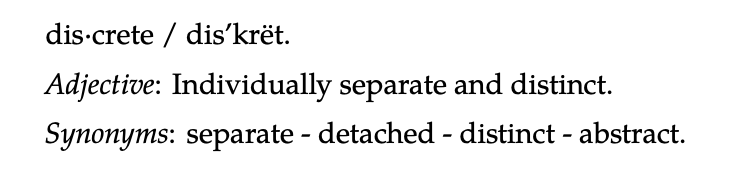
\includegraphics[width=0.9\textwidth]{images/what_is_discrete_math} \\
\end{center}
\pause 
\vspace{1cm}
\begin{center}
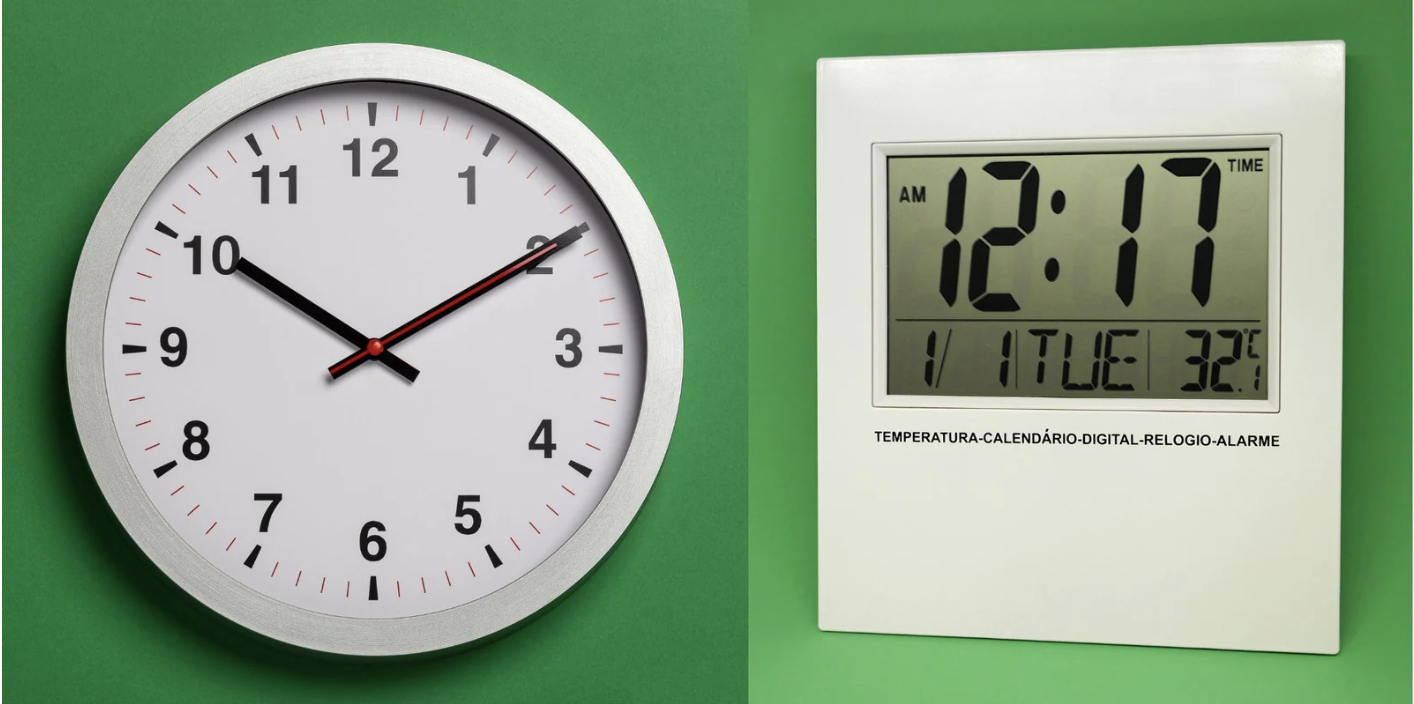
\includegraphics[width=0.6\textwidth]{images/clocks}
\end{center}
\end{frame}


\begin{frame}{Syllabus Review}

\Large \centering
See \color{blue} \underline{\href{https://montana.instructure.com/courses/20155/pages/home-page}{Canvas}} \color{black} for syllabus.

\end{frame}

 
\begin{frame}{Why Active Learning?}


\begin{figure}[h!]
    \centering

    \begin{subfigure}{0.5\textwidth}
        \centering
        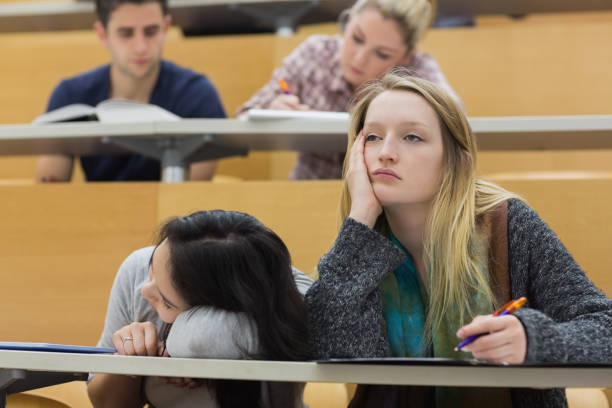
\includegraphics[width=.9\textwidth]{images/bored_student} 
    \end{subfigure}

    \vspace{1cm}
    
    \begin{subfigure}{0.45\textwidth}
        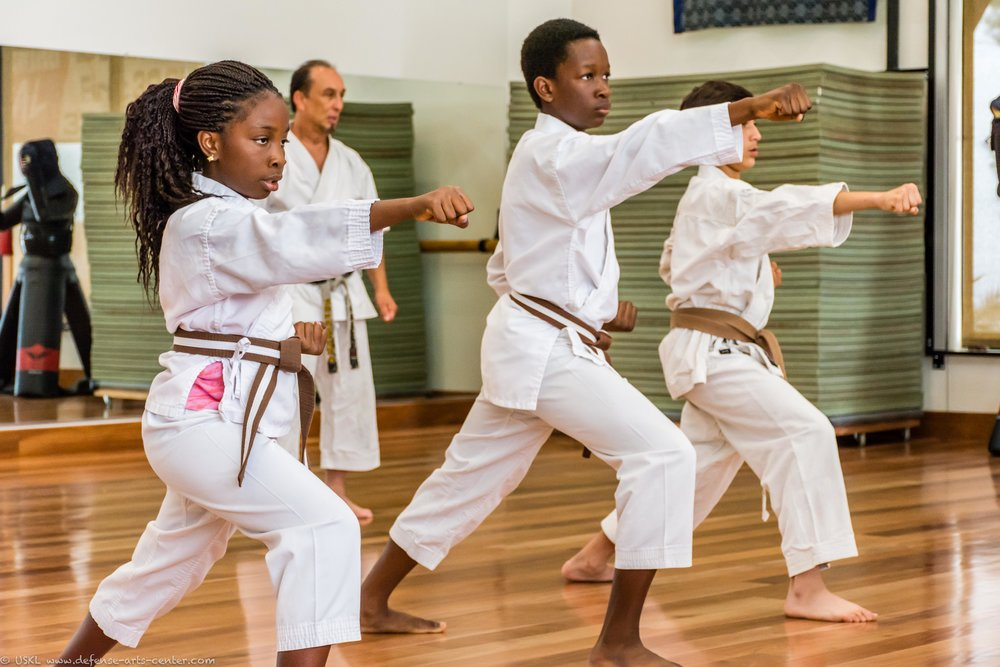
\includegraphics[width=0.9\textwidth]{images/karate} 
 
    \end{subfigure}
    \hfill
    \begin{subfigure}{0.45\textwidth}
        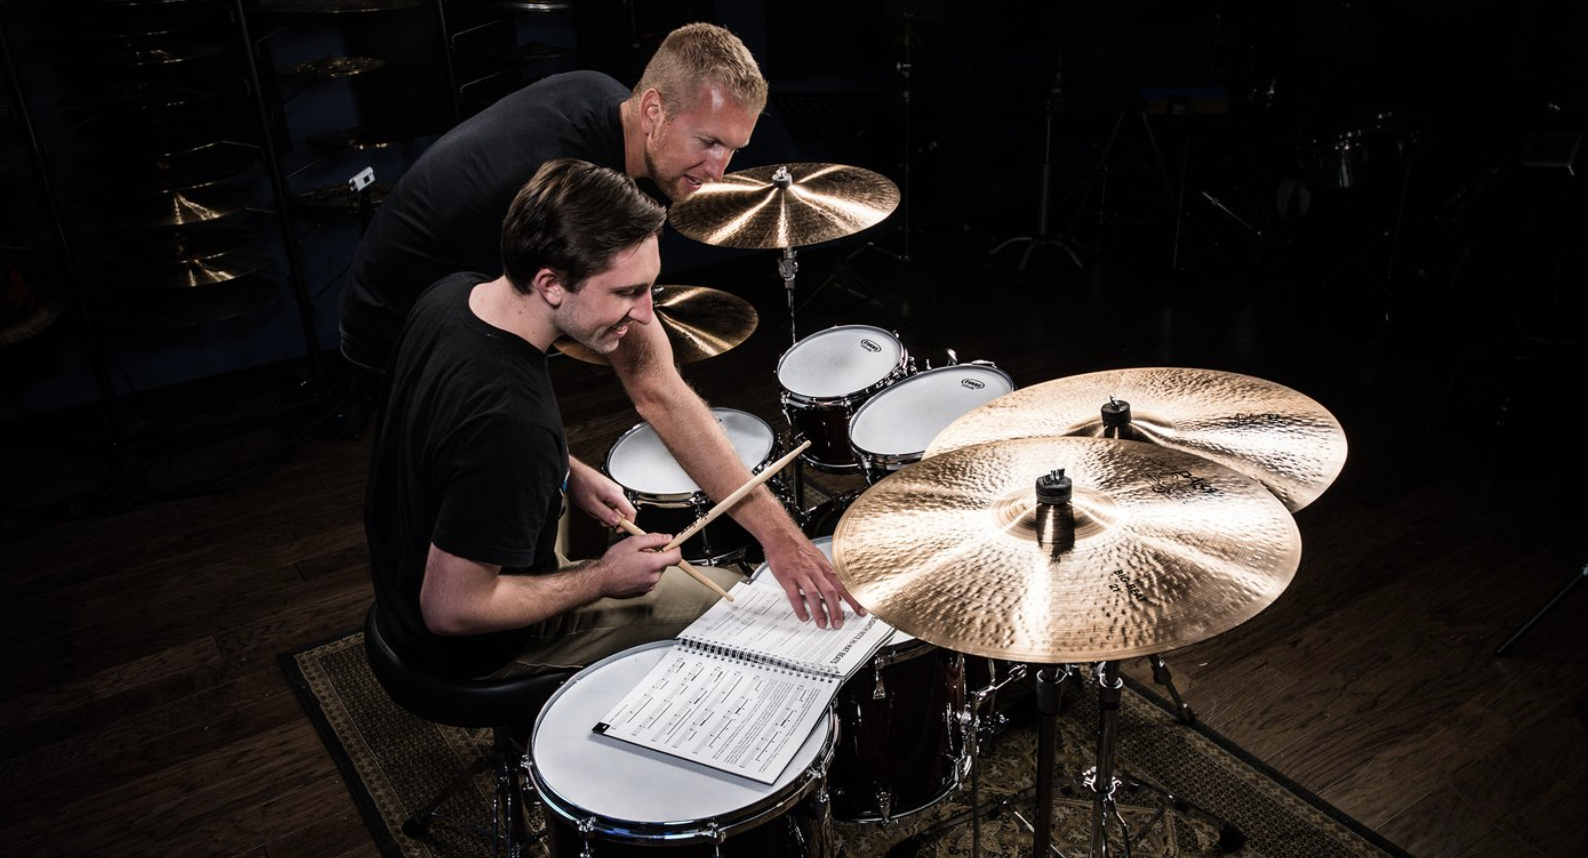
\includegraphics[width=0.9\textwidth]{images/drums} 

    \end{subfigure}
    
\end{figure}
	
\end{frame}




\begin{frame}{Why Active Learning?}
    \begin{figure}
        \centering
        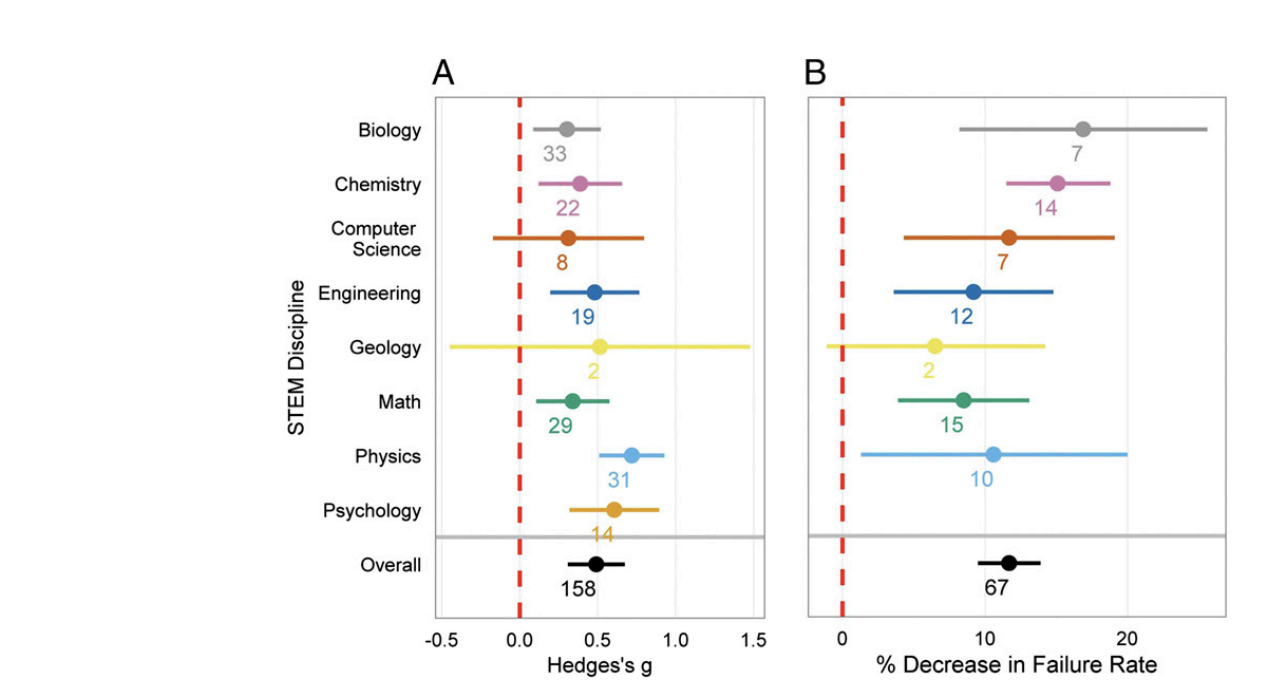
\includegraphics[width=\textwidth]{images/active_learning} 
    \end{figure}
	\citebottom{\hfill Freeman et al. (2014). \textit{Proceedings of the National Academy of Sciences}. \hfill }
\end{frame}



\begin{frame}
\begin{figure}
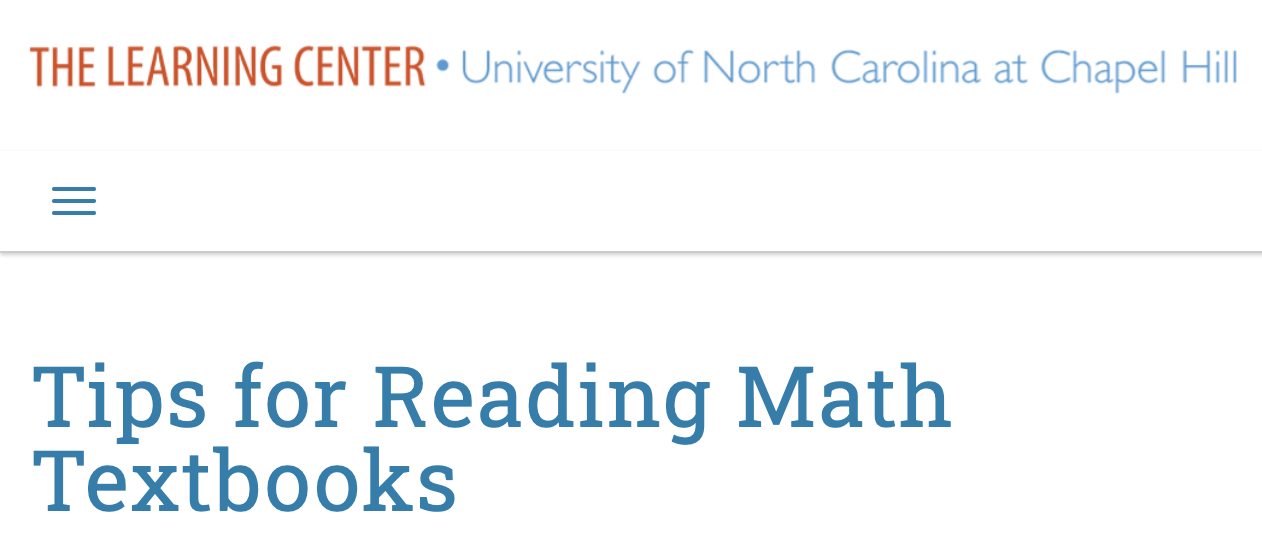
\includegraphics[width=0.7\textwidth]{images/tips_for_reading_math}
\end{figure}
%
\begin{figure}
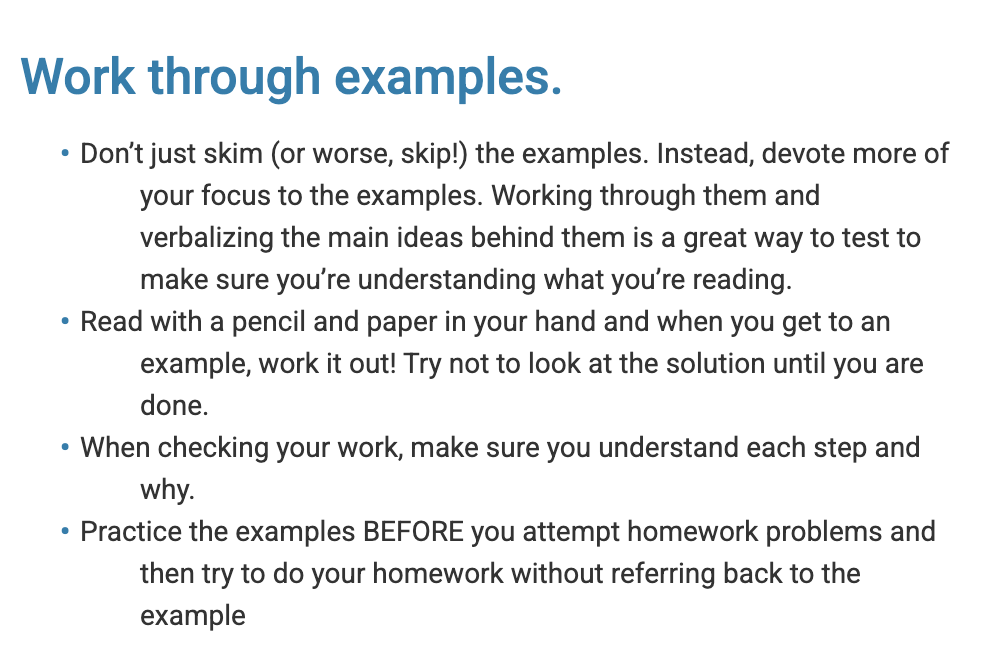
\includegraphics[width=0.7\textwidth]{images/work_through_examples}
\end{figure}
\bottomtext{\hfill Source: \url{https://learningcenter.unc.edu/tips-and-tools/readingmathtexts/}.}
\end{frame}




\begin{frame}[standout]
Virtues of discrete math -- a brief example
\end{frame}



\begin{frame}{About Me}
    \begin{columns}[T,onlytextwidth]
        \begin{column}{0.58\textwidth}
            \centering
        	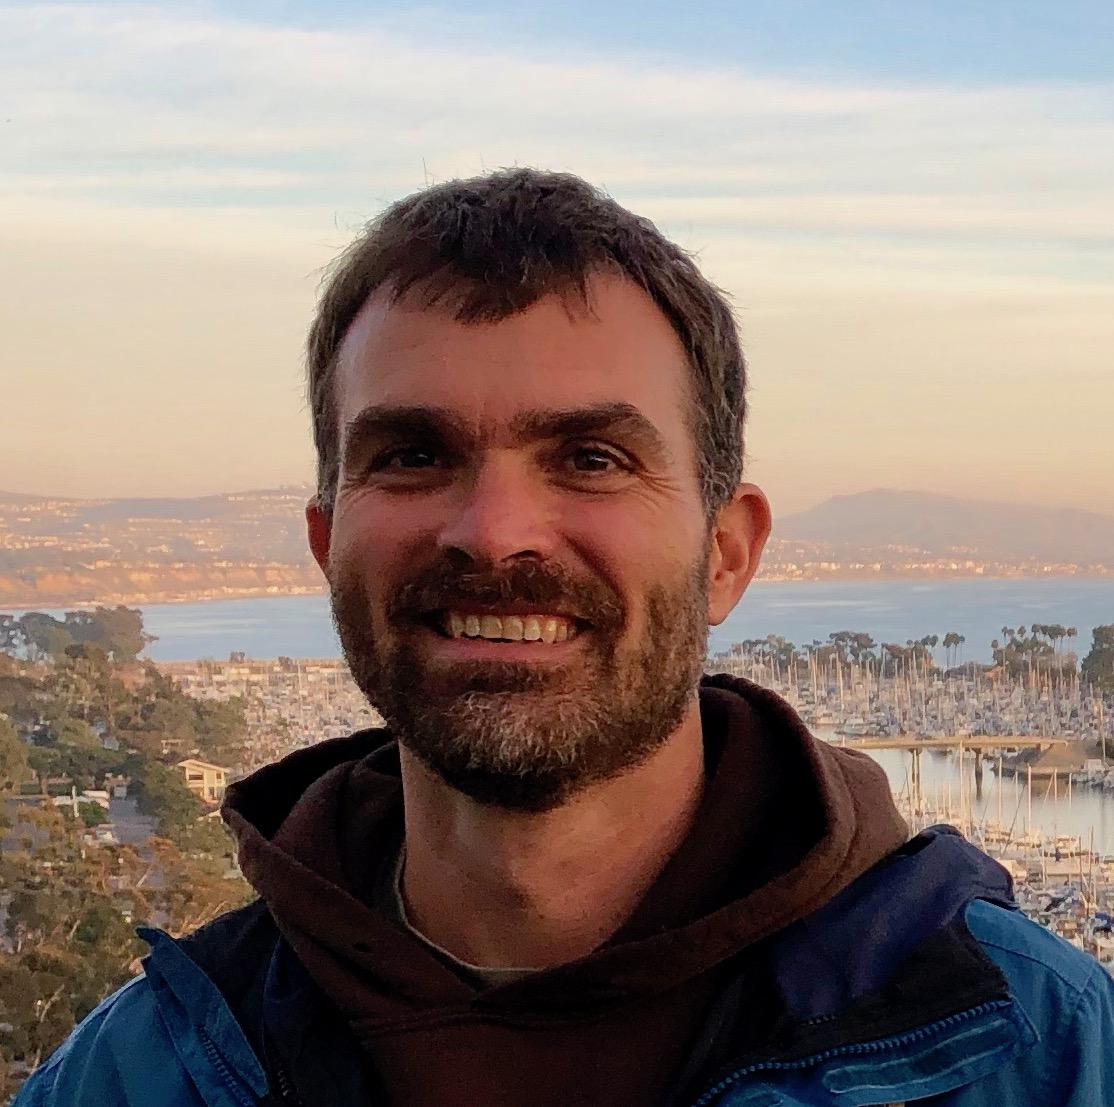
\includegraphics[width=4cm]{images/profile.jpeg}
            \vfill
            Michael Wojnowicz \\
            Assistant Professor, GSOC @ MSU \\
            Research Associate, Biostats @ Harvard \\
            Postdoc, CS @ Tufts  \\
			Distinguished Data Scientist @ Cylance \\
			(cybersecurity start-up, sold for \$1.4b) 
        \end{column}
        \begin{column}{0.38\textwidth}
            \centering
            \vspace{0.5in}\textbf{Research interests}
            \begin{itemize}
            \item Probabilistic machine learning
            \item Scalable inference
            \item Modeling spatiotemporal data	
            \end{itemize}
%           
        \end{column}
    \end{columns}
\end{frame}

%\begin{frame}{Three research themes}
%    \begin{tabular}{{p{0.15\linewidth}p{0.85\linewidth}}}
%       \centering 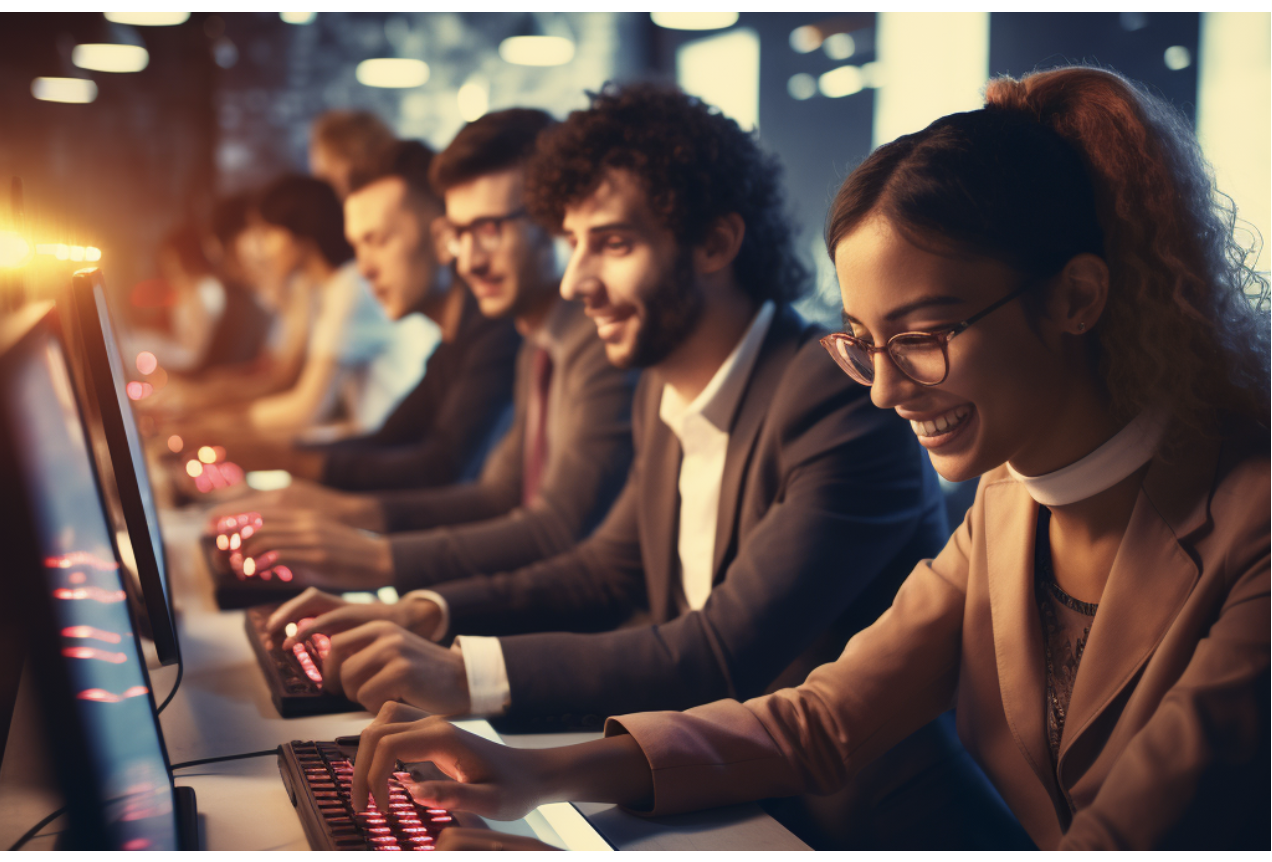
\includegraphics[width=.15\textwidth]{images/cont_auth} &
%      %First row second column
%      \colorbox{lightred}{\begin{minipage}[c]{\textwidth}\textbf{\enquote{Support Broadening} For Fast, Reliable Inference}\\
%      $\bigcdot$ Modeling 1000's of categories \; \scripttext{(\textbf{Woj.} et al., 2022, \textit{ICML})}\\
%   	  $\bigcdot$ New framework for approx. inference \; \scripttext{(\textbf{Woj.} et al., 2023, \textit{AABI})}\\ 
%      \end{minipage}}
%       \vfill \\
%      \centering  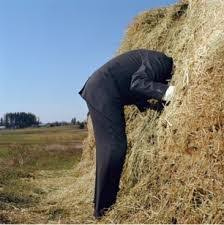
\includegraphics[width=.12\textwidth]{images/needle_in_haystack}& 
%      %2nd row second column
%            \begin{minipage}[c]{\textwidth}\textbf{Prioritization Methods: Some of Many}\\
%      $\bigcdot$ Scaling up  influence scores \; \scripttext{(\textbf{Woj.} et al., 2017, \textit{IEEE Big Data})}\\
%    $\bigcdot$ Multi-sample changepoint modeling\; \scripttext{(\textbf{Woj.} \& Miller, 2024, \textit{NESS})}\\ 
%   	  %$\bigcdot$ Anomalous segment selection \; \scripttext{(\textbf{Woj.} \& Miller, 2024, \textit{NESS})}\\ 
%      \end{minipage}
%       \vfill \\
%	\centering 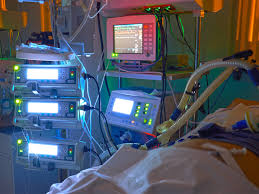
\includegraphics[width=.15\textwidth]{images/icu_monitor} & 
%    %3rd row second column
%\begin{minipage}[c]{\textwidth}\textbf{Interpretable Models for Large, Complex Temporal Data}\\
%      $\bigcdot$ Modeling \enquote{team} dynamics \; \scripttext{(\textbf{Woj.} et al., 2024, \textit{In Prep})}\\
%   	  $\bigcdot$ Modeling health care data: Multiple heterogeneous sensors, \\ irregular timestamps, and non-ignorable  missingness \\
%   	  \hfill \scripttext{(Rath, \textbf{Woj.}, \& Hughes, 2024, \textit{Submitted})}, \scripttext{(\textbf{Woj.}, et al. \textit{In prep.})}\\ 
%      \end{minipage}
%        \vfill \\
%    \end{tabular}
%\end{frame}



\begin{frame}{Motivation}

\begin{columns}[c,onlytextwidth]
    \begin{column}{0.48\textwidth}
        \centering
		\begin{figure}
	   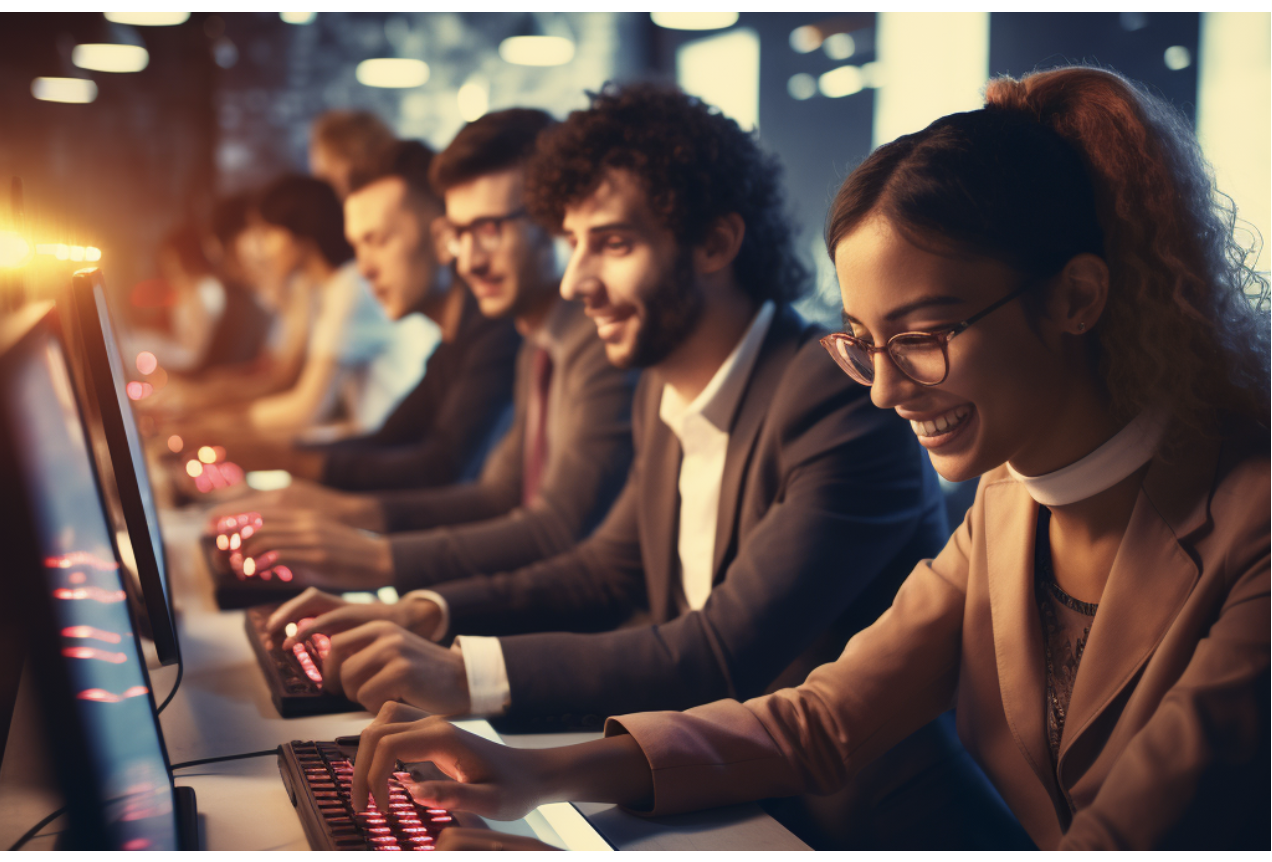
\includegraphics[width=0.9\textwidth]{images/cont_auth}
	   \vfill 
	   \textbf{Continuous authentication}:  continuously verify a user’s identity as being authentically theirs throughout their entire interaction with a digital system. 
		\end{figure}
    \end{column}
    \pause 
    \begin{column}{0.48\textwidth}
        \centering
		\vfill 
	  \begin{tabular}{cc}
	 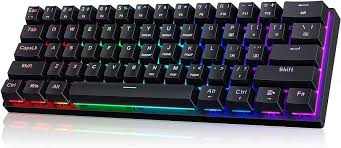
\includegraphics[width=0.5\textwidth]{images/keyboard} & 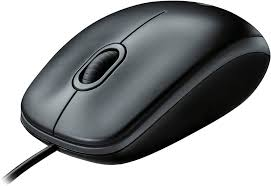
\includegraphics[width=0.5\textwidth]{images/mouse} 
	  \\
 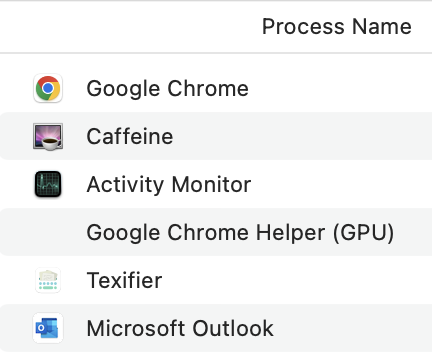
\includegraphics[width=0.5\textwidth]{images/activity_monitor} &
  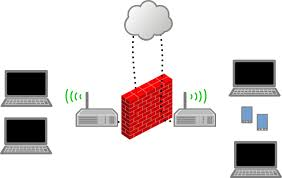
\includegraphics[width=0.5\textwidth]{images/network_traffic} 	
	  \end{tabular}
		\textbf{Data sources}: Keystrokes, \\
		mouse movements, \\ process starts, network traffic, etc.
    \end{column}
 \end{columns} 
 \pause 
 \vfill 
 \vfill 
 \textbf{Modeling Desiderata}: fast, lightweight, reliable training; interpretable probabilistic (but expressive) models 
\end{frame}




\begin{frame}{Motivation}

\begin{columns}[T,onlytextwidth]
    \begin{column}{0.48\textwidth}
        \centering
		\begin{figure}
	   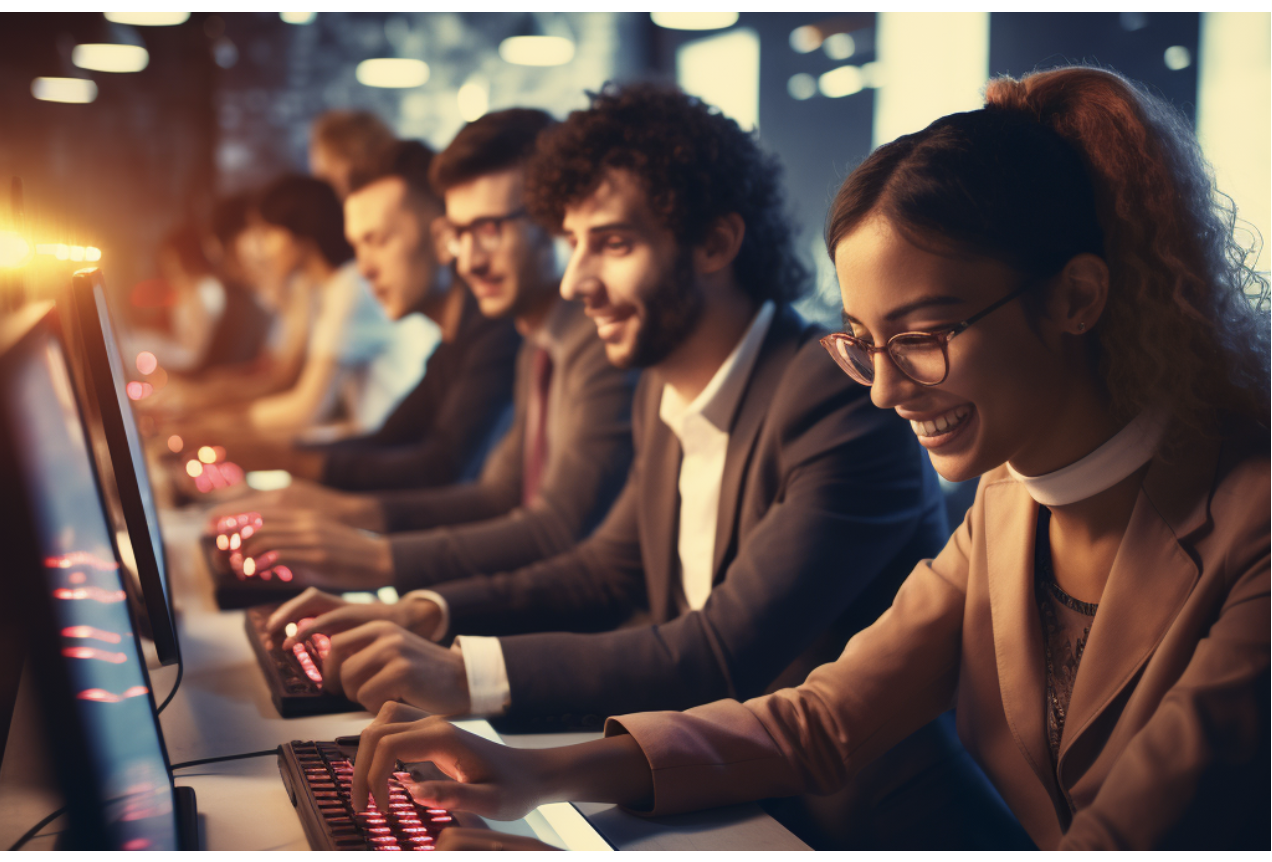
\includegraphics[width=0.9\textwidth]{images/cont_auth}
	   \vfill 
	   \textbf{Continuous authentication}:  continuously verify a user’s identity as being authentically theirs throughout their entire interaction with a digital system. 
		\end{figure}
    \end{column}
    \begin{column}{0.48\textwidth}
        \centering

	  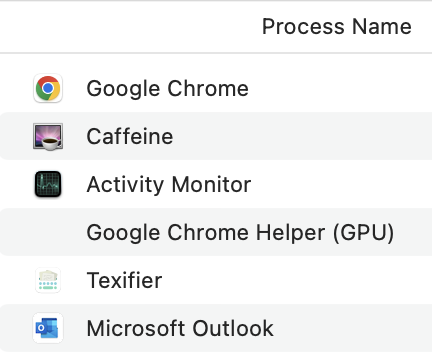
\includegraphics[width=0.9\textwidth]{images/activity_monitor} \\
	  \vfill 
		\textbf{Subgoal}: Learn computer process start sequences which characterize the typical behavior of a user.
    \end{column}
 \end{columns} 
 \pause
 \vfill 
 \textbf{Difficulty:} Many 1000s of computer processes, sparsely observed. 
\end{frame}


\begin{frame}{Solution: Scalable Bayesian Categorical Modeling}
\pause 
\begin{figure}
\centering
\caption{A new model for a computer user's process starts (with 1,553 categories, 1,553 covariates, and 17,724 examples), to aid in   \textbf{intruder detection}.} 
\pause 
\begin{tabular}{ cl}
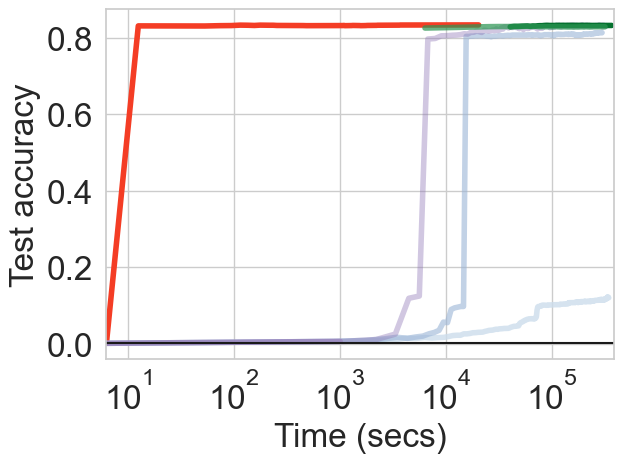
\includegraphics[height=2.3cm]{images/perf_over_time/test_accuracy_cyber_346_show_CB_logit=True_legend=False.png}  
& 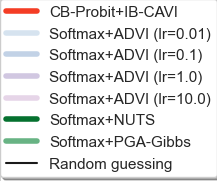
\includegraphics[height=2.3cm]{images/perf_over_time/legend_only_show_CB_logit=False.png} \\
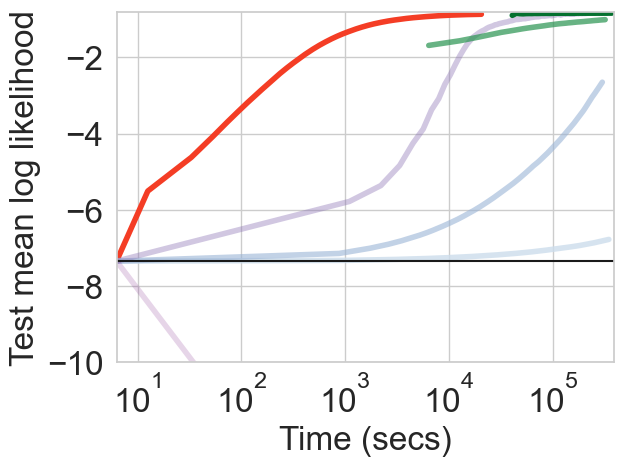
\includegraphics[height=2.8cm]{images/perf_over_time/test_mean_log_likelihood_cyber_346_show_CB_logit=True_legend=False.png} & 
\end{tabular}
\label{fig:evaluation}
\end{figure}
{\tikz[remember picture,overlay]{
        \node [draw, rectangle callout, fill=blue!10, align=left, callout relative pointer={(1,0)}, callout pointer shorten=.7cm]  at (0.4, 5.3) {\footnotesize Indistinguishable \\ \footnotesize accuracy.};}}%
{\tikz[remember picture,overlay]{
        \node [draw, rectangle callout, fill=blue!10, align=left, callout relative pointer={(1,0)}, callout pointer shorten=.7cm]  at (0.4, 2.3) {\footnotesize Little-to-no \\ \footnotesize cost in \\ \footnotesize probabilities.};}}%       
{\tikz[remember picture,overlay]{
        \node [draw,  rectangle callout, fill=red!10, align=left, callout relative pointer={(0,-1)}, callout pointer shorten=.9cm]  at (3.95,1.5) {\tiny 15 mins};}}%
{\tikz[remember picture,overlay]{
        \node [draw,  rectangle callout, fill=red!10, align=left, callout relative pointer={(0,-1)}, callout pointer shorten=.9cm]  at (5.2,1.5) {\tiny 24 hrs.};}}%
{\tikz[remember picture,overlay]{
        \node [draw,  rectangle callout, fill=red!10, align=left, callout relative pointer={(-1,0)}, callout pointer shorten=.7cm]  at (9.75,5.7) {\scriptsize A new model}}}%
%
%\pause 
%{\tikz[remember picture,overlay]{
%        \node [draw,  rounded rectangle, fill=green!10, align=left]  at (8.20, 1.8) {\footnotesize These are the results even \\ \footnotesize \textit{before} exploiting parallelism.};}}%
%\footnotesize 
%\red{Our method} delivers \textbf{similar predictive performance} in \textbf{far less time}. \\
%Bio Application: Scalably modeling genetic mutation channels
\bottomtext{\hfill Wojnowicz, Miller, Aeron, Hughes, `22, \textit{International Conference of Machine Learning (ICML)}.}
\end{frame}



\begin{frame}[standout]

\large \centering
The solution to this problem used almost every content area we're covering in this course

\vfill 
\begin{itemize}
	\item Discrete probability 
	\item Counting
	\item Complexity (Big-O notation)
	\item Recursions
	\item Graph theory
	\item Proof techniques
\end{itemize}
\end{frame}



\begin{frame}{Virtues of developing mathematical reasoning (generally)}

\begin{itemize}
\item Enhances performance studying \textit{any} domain -- not only computer science, but also cybersecurity, sociology, etc.  \pause 
\item Enhances performance at work -- often, math gets the job done better. \pause 
\item \$\$\$ \pause 
\end{itemize}

\end{frame}


\begin{frame}{Don't like math?:  Tips for success}

\begin{itemize}
	\item Be open-minded!  Don't stereotype yourself. \pause  % Tell story of how a Floridian learned to love Bozeman
	\item \textit{Growth mindset}: Anyone can improve from where they are.   \pause
	\item \textit{Culture of confusion}: It's great to be wrong! That's how we learn.  \pause 
	\item Take solace: We're starting from scratch. (No calculus!) \pause
	\item Stay on track by doing daily assignments. \pause 
	\item Use resources (office hours, tutoring, classmates, etc.) \pause 
	\item Contact me early if you're struggling.  I'm here to help! \pause 
\end{itemize}

\end{frame}




%
%\begin{frame}{Virtues of developing mathematical reasoning}
%    \begin{figure}
%        \centering
%        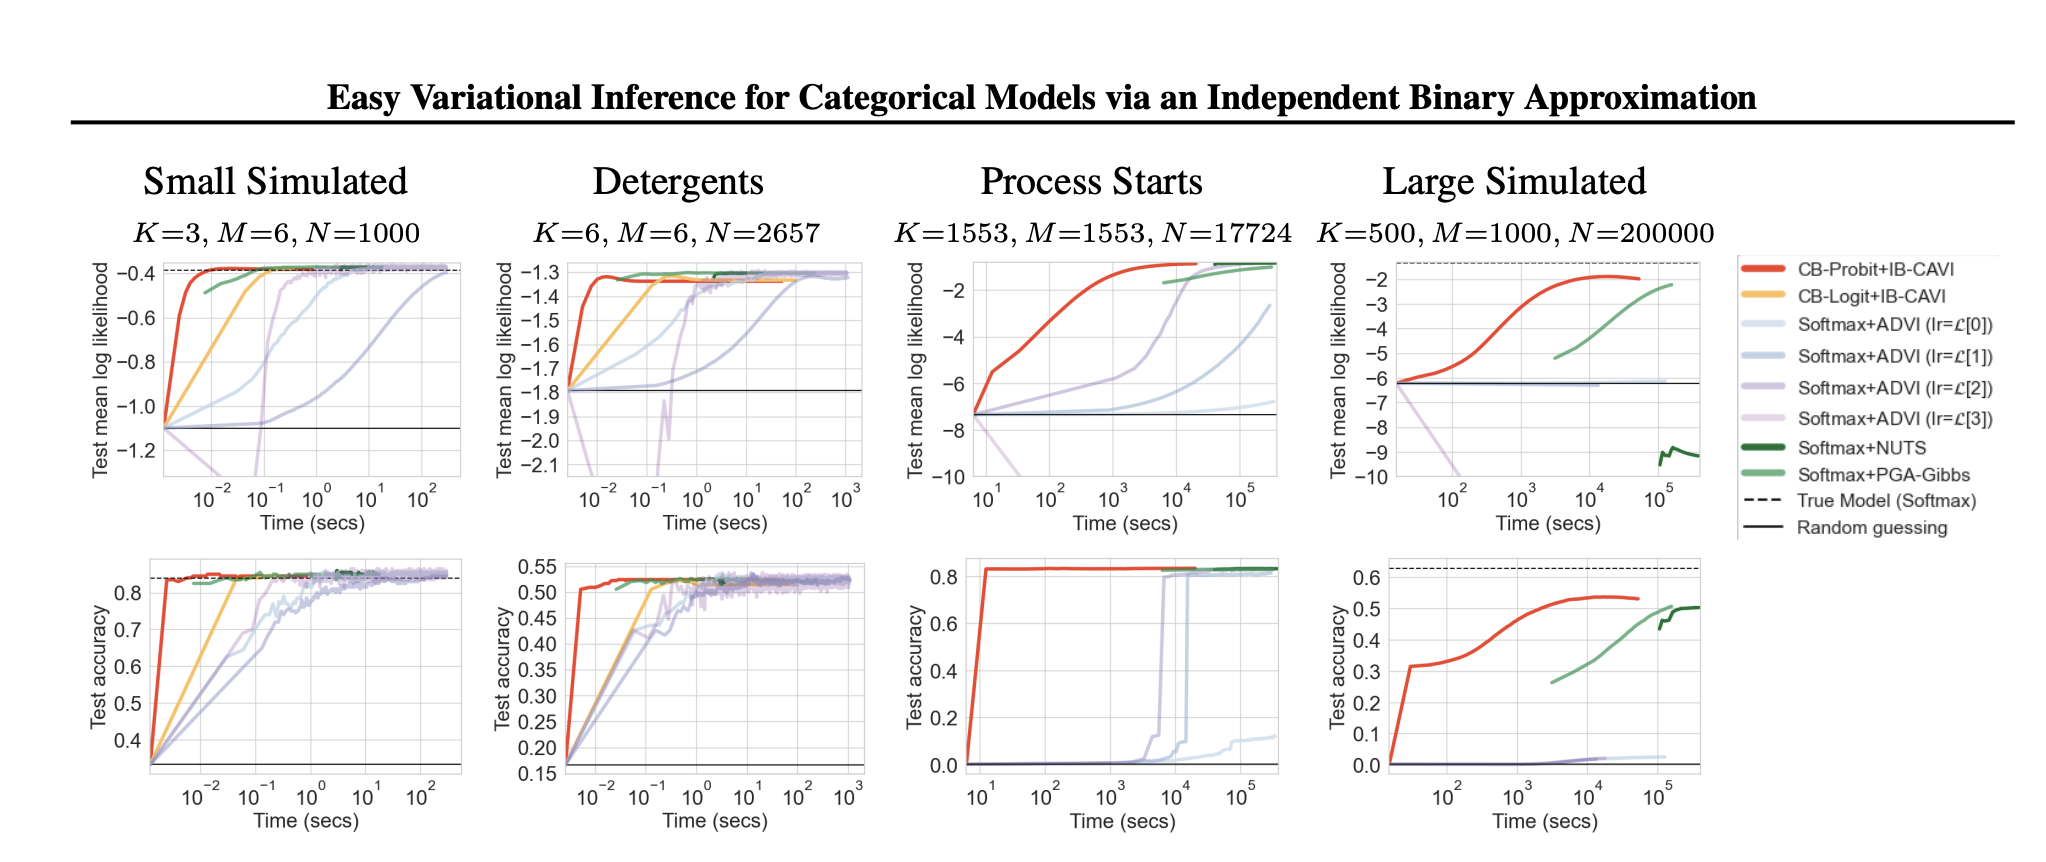
\includegraphics[width=.9\textwidth]{images/icml} 
%    \end{figure}
%   \citebottom{\hfill Wojnowicz et al. (2022). \textit{International Conference of Machine Learning (ICML)}. \hfill }
%	
%\end{frame}



%\begin{frame}{Discrete math: Example application}
%
%
%Find subtle DNA copy number alterations to support \textbf{early cancer detection}.
%
%\centering \includegraphics[width=.2\textwidth]{images/amplification_deletion} 
%
%\citebottom{Image from: Nabavi \& Zare (2022).}
%
%\end{frame}
%
%
%\begin{frame}
%\begin{columns}[T,onlytextwidth]
%    \begin{column}{0.4\textwidth}
%        \centering
%        \vspace{1in}
%        \Large How to detect changepoints within heavy noise?
%     \end{column}
%    \begin{column}{0.6\textwidth}	
%	 \begin{center}
%	  \includegraphics[width=0.5\linewidth]{images/sample_0} \\
%	\includegraphics[width=0.5\linewidth]{images/sample_1}
%	\end{center}
%    \end{column}
%\end{columns}
%
%\end{frame}
%
%
%\begin{frame}
%
%\large \centering
%The solution to this problem uses almost every content area we're covering in this course
%
%\vfill 
%\begin{itemize}
%	\item Discrete probability 
%	\item Counting
%	\item Complexity (Big-O notation)
%	\item Recursions
%	\item Graph theory
%	\item Proof techniques
%\end{itemize}
%\end{frame}

\end{document}


\end{document}